
\chapter{系统实现和实验结果}
\label{chap:experiment}

\section{系统具体实现}
\label{sec:implementation}
我们采用Scala语言来搭建我们的系统。Scala是一种运行在JVM上的静态语言,支持函数式、
面向对象等多种编程范式,可以和Java代码无缝地进行交互。目前Scala还处于不断发展中,
新版本不向后兼容,我们的系统在Scala 2.10上可以编译通过。在工程管理上,我们使
用sbt管理Scala代码的编译和依赖关系。

在系统的实现中我们还使用了许多第三方库,除了在第~\ref{chap:cluster}章中介绍
的Actor库Akka,还有:
\begin{itemize}
\item 日志系统:基于twitter公司开源的util包,地址在
  \url{https://github.com/twitter/util}。
\item 配置文件读取:基于typesafe的config包,地址
  在\url{https://github.com/typesafehub/config}。
\item 网页字符集检测:ICU4J,地址在\url{http://site.icu-project.org},这是一
  套UNICODE相关的工具集,提供了较好的字符集编码检测功能,我们用于检测中文网页的字
  符集。
\item HTML解析器:jsoup,地址在\url{http://jsoup.org},是一个用Java语言实现
  的HTML解析器,用于DOM Tree的构建和节点内容的抽取。
\end{itemize}
\section{模板匹配演示系统}
\label{sec:demo}
为了直观地显示网页模板的匹配效果,我们基于Play! Framework的Web开发框架实现了一
个Web Service,用于实验的演示。该Web Service的工作原理
如\reffig{experiment:fig:demo}所示。
\begin{figure}
  \centering
  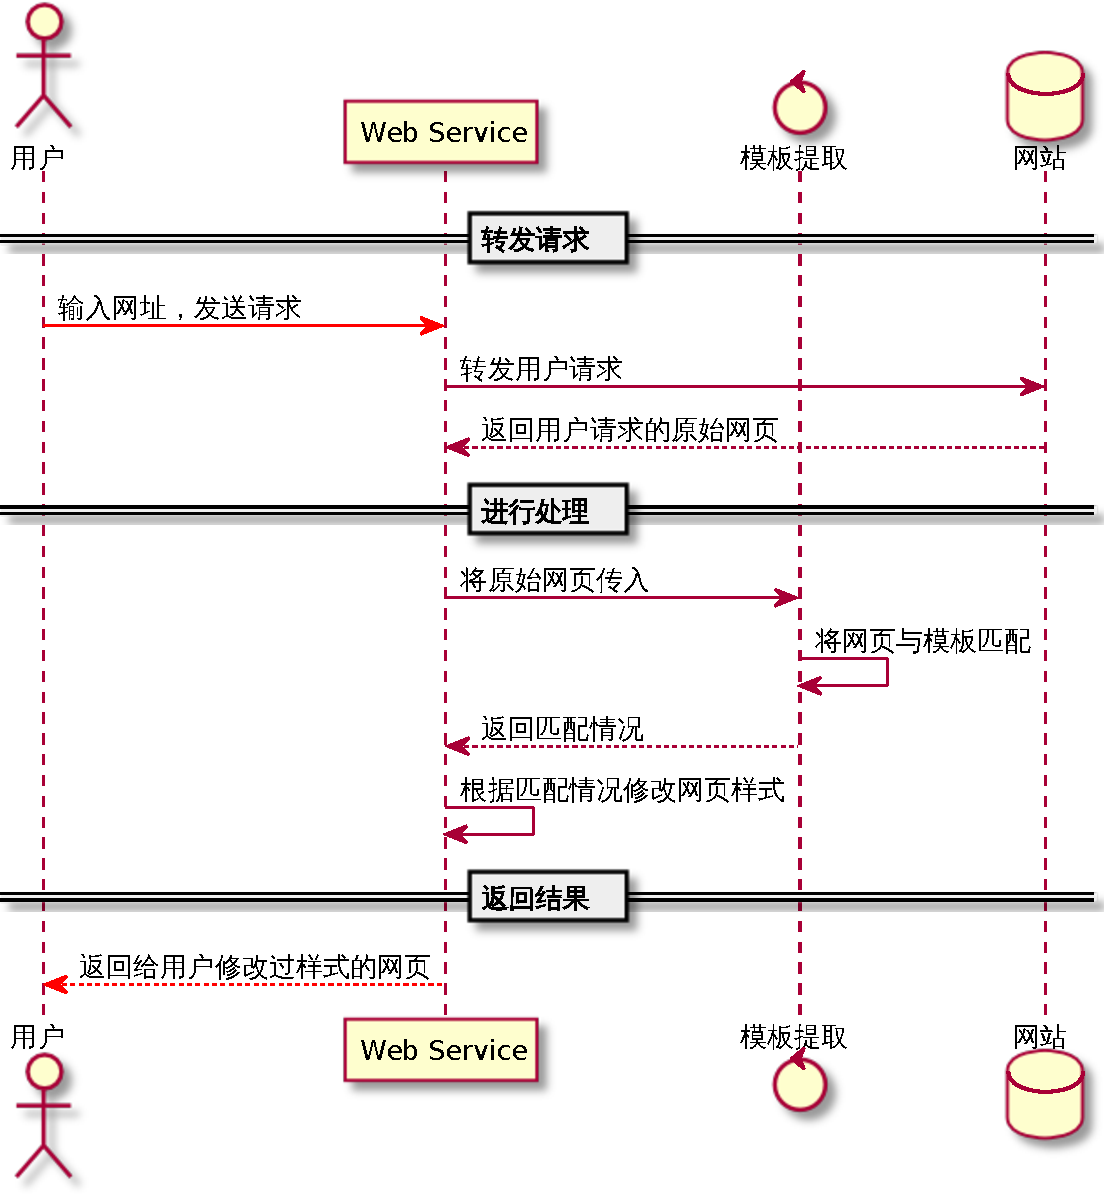
\includegraphics[width=0.75\textwidth]{experiment06/demo}
  \caption{Web Service工作原理}
  \label{experiment:fig:demo}
\end{figure}

用户需要输入一个用于和系统的模板进行匹配的网页的URL,系统返回给用户一个修改了样式
的新的网页,其中原网页和模板匹配上的部分会有和其他部分不同的显示效果,这样用户就
可以通过浏览器中直观地看到模板的匹配效果。

实验演示的效果如\reffig{experiment:fig:demoresult}所示。每个被突出显示的区域为我
们要抽取的内容,鼠标悬浮时提示对应的字段名字。
\begin{figure}[h]
  \centering
  
\includegraphics[width=0.75\textwidth]{experiment06/demo-output-new}
  \caption{实验演示系统效果}
  \label{experiment:fig:demoresult}
\end{figure}

\section{实验和分析}
\label{sec:result-analysis}

\subsection{实验环境和数据}
\label{sec:dataenv}
我们实验所用的机器的配置情况是:16个逻辑核的CPU,24G内存,操作系统为64位的CentOS。
后续的实验均在这个机器上进行。

我们有两个实验数据集,分别为博客(blog)和新闻(news)。实验数据集的概况
如\reftbl{experiment:tab:overview}所示。
\begin{table}[h]
  \centering
% BEGIN RECEIVE ORGTBL 实验数据概况
\begin{tabular}{lll}
  \toprule
 & blog & news \\
\hline
文件个数 & 59998 & 81561 \\
总大小 & 5.4G & 7.9G \\
来源 & blog.sina.com.cn & ent.sina.com.cn \\
\bottomrule
\end{tabular}
% END RECEIVE ORGTBL 实验数据概况
  \caption{实验数据概况}
  \label{experiment:tab:overview}
\end{table}
\begin{comment}
#+ORGTBL: SEND 实验数据概况 orgtbl-to-latex :splice nil :skip 0
|          | blog             | news            |
|----------+------------------+-----------------|
| 文件个数 | 59998            | 81561           |
| 总大小   | 5.4G             | 7.9G            |
| 来源     | blog.sina.com.cn | ent.sina.com.cn |
\end{comment}

接下来的几个小节我们将大体按照模块的顺序,依次介绍实验的详细情况。
\label{sec:results}
\subsection{预处理模块实验与分析}
\label{sec:experiement:pre}
在预处理模块中,我们首先将从原始的网页集合中过滤掉无用的网页,包括目录页和错误页,
采用的是第~\ref{sec:filterintro-useless}节中介绍的基于规则的方
法。\reftbl{experiment:tab:filter}给出了实验中使用的过滤规则和过滤后的结果。
\begin{table}[h]
  \centering
% BEGIN RECEIVE ORGTBL 过滤无用网页
\begin{tabular}{lrr}
  \toprule
 & blog & news \\
\hline
目录页URL规则 & .*(?<!\textbackslash\textbackslash.html?)\$ & .*(?<!\textbackslash\textbackslash.s?html)\$ \\
错误页最大长度 & 6000 & 6000 \\
原来总文件个数 & 59998 & 81561 \\
过滤后详细页个数 & 35466 & 65655 \\
\bottomrule
\end{tabular}
% END RECEIVE ORGTBL 过滤无用网页
  \caption{过滤无用网页实验结果}
  \label{experiment:tab:filter}
\end{table}
\begin{comment}
#+ORGTBL: SEND 过滤无用网页 orgtbl-to-latex :splice nil :skip 0
|                  |                                       blog |                                        news |
|------------------+--------------------------------------------+---------------------------------------------|
| 目录页URL规则    | .*(?<!\textbackslash\textbackslash.html?)$ | .*(?<!\textbackslash\textbackslash.s?html)$ |
| 错误页最大长度   |                                       6000 |                                        6000 |
| 原来总文件个数   |                                      59998 |                                       81561 |
| 过滤后详细页个数 |                                      35466 |                                       65655 |
\end{comment}

过滤掉了不需要的网页以后,我们得到了详细页的集合。我们从每个详细页集合中分别随机
抽取10000个样本作为每个集合的训练集。

接下来将去除无用的标签。\reftbl{experiment:tab:uselesstags}给出了我们实验中去掉无
用标签的几种正则表达式模式及每种模式对应的标签名。
\begin{table}[h]
  \centering
% BEGIN RECEIVE ORGTBL 无用标签
\begin{tabular}{ll}
  \toprule
正则表达式模式 & 对应的标签名 \\
\hline
(?is)<tag.*?>.*?</tag> & style,script \\
(?is)<[/]?tag.*?> & link,input,br,img,meta,wbr \\
(?is)<[/]?tag.*?> & strong,em,font,b,p,li,ul,ol,td,tr,th,tbody,table \\
\bottomrule
\end{tabular}
% END RECEIVE ORGTBL 无用标签
  \caption{去掉的无用标签}
  \label{experiment:tab:uselesstags}
\end{table}
\begin{comment}
#+ORGTBL: SEND 无用标签 orgtbl-to-latex :splice nil :skip 0
| 正则表达式模式         | 对应的标签名                                     |
|------------------------+--------------------------------------------------|
| (?is)<tag.*?>.*?</tag> | style,script                                     |
| (?is)<[/]?tag.*?>      | link,input,br,img,meta,wbr                       |
| (?is)<[/]?tag.*?>      | strong,em,font,b,p,li,ul,ol,td,tr,th,tbody,table |
\end{comment}

下面我们对利用后缀树检测重复记录的算法的运行结果做一些统计。具体地,我们统计出每
个数据集中算法检测出的重复记录的长度的分布情况,每个集合的文件个数都是10000。结果
如\reftbl{experiment:tab:recordlength}所示。
\begin{table}[h]
  \centering
% BEGIN RECEIVE ORGTBL recordlength
\begin{tabular}{rrr}
  \toprule
重复记录长度 & blog & news \\
\hline
1 & 1365336 & 1278686 \\
2 & 177588 & 63475 \\
3 & 5921 & 11733 \\
4 & 1224 & 391 \\
5 & 243 & 2872 \\
6 & 95 & 22 \\
7 & 18958 & 23 \\
8 & 50 & 40 \\
9 & 60 & 356 \\
$\ge$10 & 745 & 3575 \\
\bottomrule
\end{tabular}
% END RECEIVE ORGTBL recordlength
  \caption{检测出的重复记录长度的分布情况\label{experiment:tab:recordlength}}
\end{table}
\begin{comment}
#+ORGTBL: SEND recordlength orgtbl-to-latex :splice nil :skip 0
| 重复记录长度 |    blog |    news |
|--------------+---------+---------|
|            1 | 1365336 | 1278686 |
|            2 |  177588 |   63475 |
|            3 |    5921 |   11733 |
|            4 |    1224 |     391 |
|            5 |     243 |    2872 |
|            6 |      95 |      22 |
|            7 |   18958 |      23 |
|            8 |      50 |      40 |
|            9 |      60 |     356 |
|       $>=$10 |     745 |    3575 |
\end{comment}


我们可以看到,总体上重复记录的长度比较短,大部分的重复记录集中在长
度1\textasciitilde{}3之间,其中长度为1的重复记录最多。也有个别例外情况,如blog数
据集还有较多的长度为7的重复记录。

从检测出的重复记录的个数来看,网页中有大量的重复记录,因此如果没有这一步将大量的
重复记录合并,后期的聚类和模板提取都会受到较大的影响,说明预处理的时候合并重复记
录这一步是非常重要的。
\subsection{聚类和模板生成模块实验和分析}
由于我们要处理的网页的数量非常多,计算网页的结构相似度将是我们整个系统最耗时的部
分,因此,我们先将训练集中所有的文档结构相似度离线算好,方便后续的实验。

在聚类模块中,最重要的实验参数是聚类时设置的距离阈值,距离越大,相似度越低。为了
观察该阈值对实验结果的影响,我们调整该阈值,观察聚类的个数的变化;同时,我们还将
统计根据不同的聚类结果生成的模块的一些信息,观察聚类阈值的变化对最后模板的生成有
怎样的影响。我们选择在news数据集上进行实验,具体的实验结果见\reftbl{experiment:tab:threshold}。

\begin{table}[h]
% BEGIN RECEIVE ORGTBL 阈值变化
\begin{tabular}{rrrrr}
  \toprule
距离阈值 & 聚类个数 & 必选节点平均长度 & 可选节点平均长度 & 模板平均长度 \\
\hline
0.3 & 16 & 5.18 & 2.14 & 21.8 \\
0.4 & 9 & 4.66 & 2.59 & 22.6 \\
0.5 & 7 & 4.68 & 2.71 & 24.9 \\
0.6 & 5 & 3.76 & 2.90 & 24.8 \\
\bottomrule
\end{tabular}
% END RECEIVE ORGTBL 阈值变化
\caption{阈值变化对实验结果的影响\label{experiment:tab:threshold}}
\end{table}
\begin{comment}
#+ORGTBL: SEND 阈值变化 orgtbl-to-latex :splice nil :skip 0
| 距离阈值 | 聚类个数 | 必选节点平均长度 | 可选节点平均长度 | 模板平均长度 |
|----------+----------+------------------+------------------+--------------|
|      0.3 |       16 |             5.18 |             2.14 |         21.8 |
|      0.4 |        9 |             4.66 |             2.59 |         22.6 |
|      0.5 |        7 |             4.68 |             2.71 |         24.9 |
|      0.6 |        5 |             3.76 |             2.90 |         24.8 |
\end{comment}

其中,必选节点长度定义为必选节点包含的基本节点个数;可选节点的长度定义为可选节点
对应的每个基本节点序列的加权长度和,权重为该序列的出现概率;模板的长度为必选节点
和可选节点的个数和。

从\reftbl{experiment:tab:threshold}所示的实验结果中,我们可以看到聚类时设置的阈值
大小不仅会影响聚类的个数,对后续的模板生成也有较大的影响。通过分析,我们可以得到
以下结论:聚类时的阈值越小,聚类的个数越多,也就意味着每个类的分得越细,每个类里
的点相似度越高,导致$s_{common}$越长,因此必选节点的平均长度也就越长。类似地,可
选节点的长度将变短。在序列总长度不变的情况下,必选节点越长,必选节点的个数就相应
减少,模板的平均长度也就减小。\reftbl{experiment:tab:threshold}所示的结果基本还是
符合以上分析的。

\subsection{内容抽取模块实验和分析}
为了验证我们的系统能在实际的生产环境中使用,我们在测试集上进行了实验。我们在聚类
的时候使用的距离阈值均为0.5的情况下分别生成了博客数据和新闻数据的模板。然后人工对
每个模板进行少量标注,利用标注好的模板,对每个新的网页(测试集)进行内容抽取,最
后将抽取的内容用XML格式保存下来。我们分别选取了5000个测试样本,将结果保存到
了XML中。\reffig{experiment:fig:xmloutput}是我们保存到XML中的结果的截图。
\begin{figure}[hb]
  \centering
  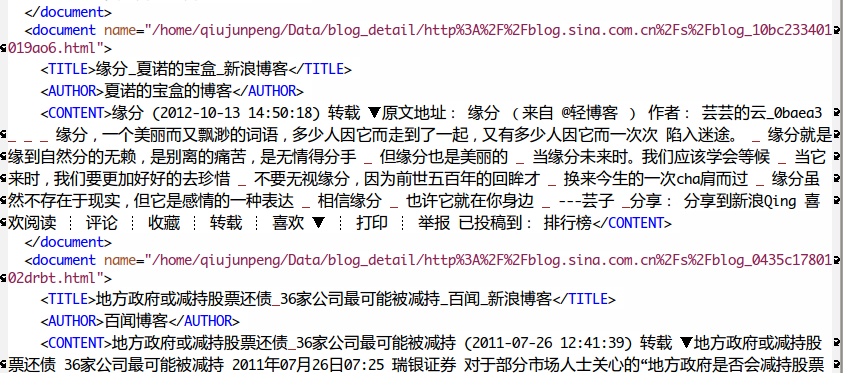
\includegraphics[width=0.8\textwidth]{experiment06/xmloutput-1}
  \caption{XML保存的结果截图}
  \label{experiment:fig:xmloutput}
\end{figure}

从实际的提取效果来看,我们的系统达到了预期的结果——只需要少量的人工标注,系统就能
自动抽取出我们需要的信息。

%%% Local Variables: 
%%% mode: latex
%%% TeX-master: "../main"
%%% End: 
